\documentclass{beamer}
\usetheme{boadilla}
%\usepackage[scale]{helvet}
\usepackage{etex}
\usepackage{helvet}

\usepackage[all]{xy}
\usepackage{color}
\usepackage{booktabs}
\usepackage{amsmath,amsthm,amssymb}

\usepackage{fancybox}
\usepackage{comment}
\usepackage{array}
\usepackage{multicol}
\usepackage{multirow}
%% I like helvetica, but here are some other font options
% \usepackage{libertine}
%\usepackage{xunicode}
%\usepackage{xltxtra}
%\usepackage{fontspec}
%\setmainfont{Minion Pro}
%\xyoption{color}
%\xyoption{frame}
%\UseCrayolaColors


\newcommand\Wider[2][3em]{%
\makebox[\linewidth][c]{%
  \begin{minipage}{\dimexpr\textwidth+#1\relax}
  \raggedright#2
  \end{minipage}%
  }%
}


\newcommand{\be}{\mathbf{e}}

\newcommand{\bC}{\mathbf{C}}
\newcommand{\bD}{\mathbf{D}}
\newcommand{\bI}{\mathbf{I}}
\newcommand{\bK}{\mathbf{K}}
\newcommand{\bS}{\mathbf{S}}
\newcommand{\bU}{\mathbf{U}}
\newcommand{\bW}{\mathbf{W}}
\newcommand{\bX}{\mathbf{X}}
\newcommand{\bx}{\mathbf{x}}
\newcommand{\bY}{\mathbf{Y}}
\newcommand{\bZ}{\mathbf{Z}}

\newcommand{\bmu}{\boldsymbol\mu}

\newcommand{\bSigma}{\boldsymbol\Sigma}
\newcommand{\bzero}{\mathbf{0}}
\newcommand{\bone}{\mathbf{1}}

\setbeamertemplate{footline}{
\leavevmode%
\hbox{%
\begin{beamercolorbox}[wd=.15\paperwidth,ht=2.25ex,dp=1ex,center]{author in head/foot}%
    \usebeamerfont{title in head/foot}Boca, Leek
\end{beamercolorbox}%
\begin{beamercolorbox}[wd=.6\paperwidth,ht=2.25ex,dp=1ex,center]{title in head/foot}%
    \usebeamerfont{title in head/foot}\insertshorttitle
\end{beamercolorbox}%
\begin{beamercolorbox}[wd=.25\paperwidth,ht=2.25ex,dp=1ex,right]{date in head/foot}%
    \usebeamerfont{date in head/foot}\insertshortdate{}\hspace*{2em}
    \insertframenumber{} / \inserttotalframenumber\hspace*{2ex} 
\end{beamercolorbox}}%
\vskip0pt%
}
\makeatother

\setbeamertemplate{navigation symbols}{}%remove navigation symbols


\title{A direct approach to estimating false discovery rates conditional on covariates}
\author{Simina Boca$^1$, Jeff Leek$^2$}
\date{July 31, 2017}
\institute{$^1$Georgetown University Medical Center, $^2$Johns Hopkins Bloomberg School of Public Health\\ \vspace{0.5cm}
\normalsize \url{https://github.com/SiminaB/Presentations}\\ \vspace{1.5cm}
\large Joint Statistical Meetings, Baltimore, MD}

\begin{document}

%\begin{frame}[plain,t,noframenumbering]
%\Wider[4em]{
%\includegraphics[scale=0.55]{John_Storey_slides.png} 
%}
%\end{frame}

%%%%%%%%%%%%%%%%%%%%%%%%%
%%%%%%%%%%%%%%%%%%%%%%%%%
%%%%%%%%%%%%%%%%%%%%%%%%%

\begin{frame}[plain,t,noframenumbering]
\titlepage
\end{frame}

%%%%%%%%%%%%%%%%%%%%%%%%%
%%%%%%%%%%%%%%%%%%%%%%%%%
%%%%%%%%%%%%%%%%%%%%%%%%%

\begin{frame}
\frametitle{Goal}

Extend {\color{red}false discovery rate framework} to easily
incorporate {\color{red}external covariates (meta-data)} in decision of whether to reject a hypothesis when testing many hypotheses at once.

\end{frame}

%%%%%%%%%%%%%%%%%%%%%%%%%
%%%%%%%%%%%%%%%%%%%%%%%%%
%%%%%%%%%%%%%%%%%%%%%%%%%

\begin{frame}
\frametitle{Background}

{\color{red}Multiple testing} is a ubiquitous issue in modern science:\\ \vspace{0.5cm}
Need to test relationship between hundreds or thousands of variables/features and one outcome (genomics, metabolomics etc.)

\begin{table}[ht]
\begin{tabular}{l  cc  c}
& Fail to reject null & Reject null & Total \\
\hline
Null true & $U$ & $V$ & $m_0$ \\
Null false & $T$ & $S$ & $m-m_0$ \\
\hline
& $m-R$ & $R$ & $m$
\end{tabular}
\end{table}

$R$ = number of discoveries\\
$V$ = number of false discoveries

\vspace{0.5cm}
\small Benjamini and Hochberg, 1995, \textit{JRSSB}.

\end{frame}

%%%%%%%%%%%%%%%%%%%%%%%%%
%%%%%%%%%%%%%%%%%%%%%%%%%
%%%%%%%%%%%%%%%%%%%%%%%%%

\begin{frame}
\frametitle{Background}

{\color{red}False discovery rate (FDR)} often used as framework to control for multiple testing.\vspace{0.5cm}

Natural definition:
\begin{eqnarray*}
FDR = E \left [  \frac{V}{R}  \right ].
\end{eqnarray*}
Since $R$ can be equal to $0$, usually defined as:
\begin{eqnarray*}
\label{eq:fdr}
FDR = E \left [  \frac{V}{R} \bigg| R > 0 \right ] Pr(R > 0).
\end{eqnarray*}

\small Benjamini and Hochberg, 1995, \textit{JRSSB}.


\end{frame}

%%%%%%%%%%%%%%%%%%%%%%%%%
%%%%%%%%%%%%%%%%%%%%%%%%%
%%%%%%%%%%%%%%%%%%%%%%%%%

\begin{frame}
\frametitle{Background}

FDR control and estimation approaches rely on an estimate of the proportion of null hypotheses, $\pi_0$:

\begin{eqnarray*}
\pi_0 = P(\mbox{hypothesis $i$ is null}).
\end{eqnarray*}

\begin{itemize}
\item Original Benjamini-Hochberg (BH) approach assumes $\pi_0 \equiv 1$
\item Storey, 2002, \textit{JRSSB} estimates $\pi_0$ as a fixed value and multiplies the BH FDR estimates by $\hat{\pi}_0$.
\item We expand this framework to estimate $\pi_0$ as a function of external covariates.
\end{itemize}


\end{frame}

%%%%%%%%%%%%%%%%%%%%%%%%%
%%%%%%%%%%%%%%%%%%%%%%%%%
%%%%%%%%%%%%%%%%%%%%%%%%%

\begin{frame}
\frametitle{Motivating case study}

\begin{itemize}
\item Genome-wide association ({\color{red}GWAS}) study looking at associations between millions of genetic loci and BMI (Locke et al, 2015, \textit{Nature}).
\item Loci are single nucleotide polymorphisms (SNPs) that usually have 2 possible variants (alleles).
\begin{itemize}
\item Major allele - more common allele, minor allele - less common allele.
\end{itemize}
\item Each SNP has a different population-level frequency (coded as {\color{red}MAF = minor allele frequency}).
\item Not all SNPs have the same sample size ({\color{red}N}), since they may be genotyped in different individuals.
\end{itemize}

\vspace{0.5cm}Plan to use MAF and N as external covariates!

\end{frame}


%%%%%%%%%%%%%%%%%%%%%%%%%
%%%%%%%%%%%%%%%%%%%%%%%%%
%%%%%%%%%%%%%%%%%%%%%%%%%

\begin{frame}
\frametitle{Building on prior work}

Our work builds on the work of Benjamini and Hochberg, Efron, Storey, Scott et al, 2015, \textit{JASA},
who framed the concept of {\color{red}FDR regression}, extending FDR and $\pi_0$ to include covariates.\\ \vspace{0.5cm}

We focus on estimating $\pi_0$ as a function of covariates, then using it as a plug-in estimator to estimate FDR as a function of
covariates, \`{a} la Storey.\\ \vspace{0.5cm}

We also use ideas from Ignatiadis et al, 2016, \textit{Nat. Methods} that adjusting for covariates independent of the data - conditional on 
the null being true - can improve power.

\end{frame}

%%%%%%%%%%%%%%%%%%%%%%%%%
%%%%%%%%%%%%%%%%%%%%%%%%%
%%%%%%%%%%%%%%%%%%%%%%%%%

\begin{frame}
\frametitle{Approach: Extend definitions of $\pi_0$ and FDR to include covariates}

Assume a set of covariates in a column vector $\bX_i$ of length $c$, possibly with $c=1$ and extend definitions:


\begin{eqnarray*}
\pi_0(\bx_i) &=& Pr(\theta_i = 1|\bX_i=\bx_i),\\
FDR(\bx_i) &=& E \left [  \frac{V}{R} \bigg| R > 0, \bX_i=\bx_i \right ] Pr(R > 0|\bX_i=\bx_i).
\end{eqnarray*}


\end{frame}

%%%%%%%%%%%%%%%%%%%%%%%%%
%%%%%%%%%%%%%%%%%%%%%%%%%
%%%%%%%%%%%%%%%%%%%%%%%%%

\begin{frame}
\frametitle{Motivating case study: GWAS meta-analysis for BMI}

\begin{itemize}
\item Looked at $\sim$2.5 million SNPs in $\sim$340,000 individuals, considering their association with BMI.
\vspace{0.5cm}
\item $\sim$320,000 were of European descent
\begin{itemize}
\item Used HapMap CEU population as reference for MAF
\end{itemize}
\vspace{0.5cm}
\item Sample size (N) varies between SNPs \\
(50,002 - 339,224, median = 235,717)
\end{itemize}

\end{frame}


%%%%%%%%%%%%%%%%%%%%%%%%%
%%%%%%%%%%%%%%%%%%%%%%%%%
%%%%%%%%%%%%%%%%%%%%%%%%%

\begin{frame}
\frametitle{Dependence of p-values on sample sizes}

\begin{center}
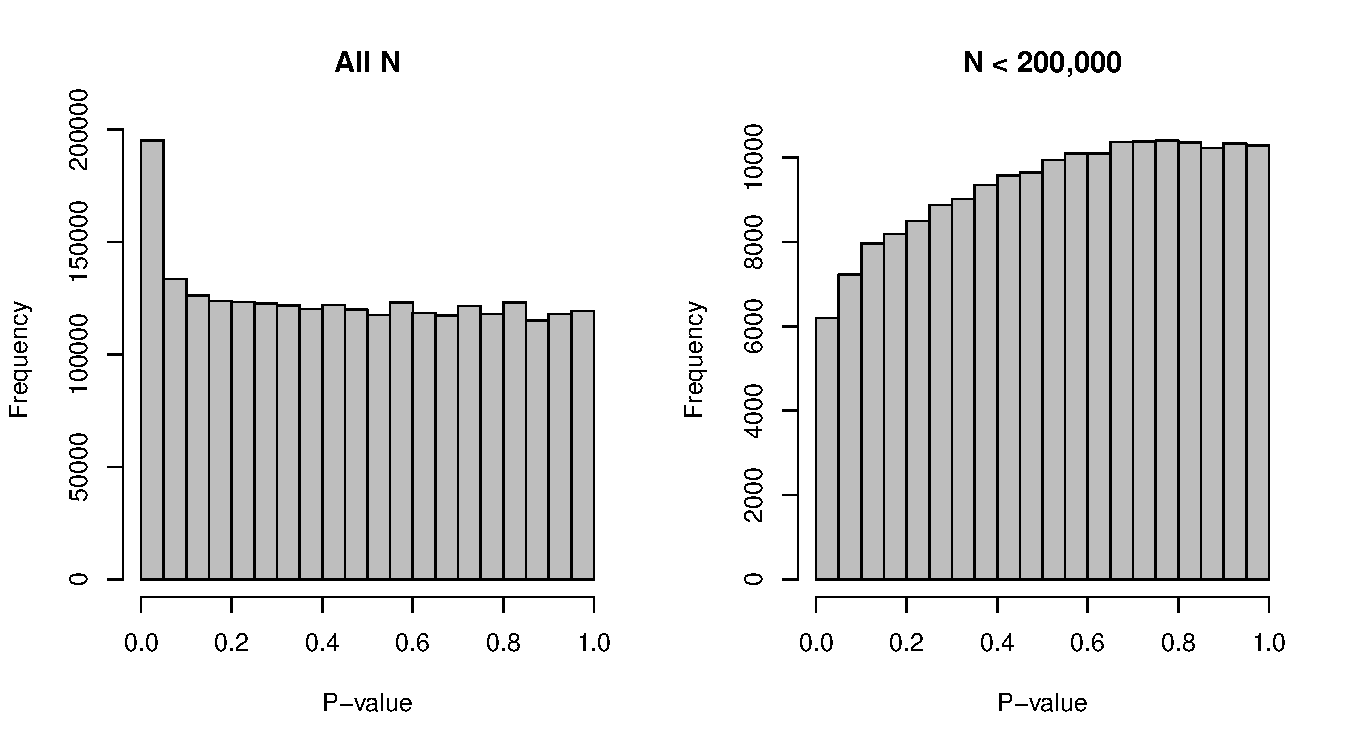
\includegraphics[scale=0.55]{Fig1-1.pdf} 
\end{center}

\end{frame}

%%%%%%%%%%%%%%%%%%%%%%%%%
%%%%%%%%%%%%%%%%%%%%%%%%%
%%%%%%%%%%%%%%%%%%%%%%%%%

\begin{frame}
\frametitle{Approach: Estimate $\pi_0(\bx_i)$ using logistic regression}

Assume that null p-values come from Uniform(0,1) and the alternative p-values from a distribution with cdf G,
so that for a large enough $\lambda \in (0,1)$, $G(\lambda) \approx 1$.

\vspace{0.5cm}
Define: $Y_i = 1(\mbox{P-value from test $i > \lambda$}) = P(\mbox{test $i$ not rejected at level $\lambda$})$.

\vspace{0.5cm}
For a fixed threshold $\lambda$:
\begin{eqnarray*}
\pi_0(\bx_i) &\approx& \frac{E[Y_i|\bX_i=\bx_i] }{1-\lambda}.
\end{eqnarray*}
Use a regression framework to estimate $E[Y_i|\bX_i=\bx_i]$, then estimate
$\pi_0(\bx_i)$ by:
\begin{eqnarray*}
\label{eq:est-pio-x}
\hat{\pi}_0(\bx_i) &=& \frac{\hat{E}[Y_i|\bX_i=\bx_i] }{1-\lambda}.
\end{eqnarray*}

\end{frame}

%%%%%%%%%%%%%%%%%%%%%%%%%
%%%%%%%%%%%%%%%%%%%%%%%%%
%%%%%%%%%%%%%%%%%%%%%%%%%

\begin{frame}
\frametitle{Approach: Estimate $\pi_0(\bx_i)$ using logistic regression}

Additional details:

\begin{itemize}
\item May need to threshold at 1, given division by $1-\lambda$.
\item Can fix $\lambda$ at e.g. 0.8 or 0.9 \textit{or} smooth over a series of thresholds $\lambda \in (0,1)$.
\item Can use a bootstrap approach for confidence intervals.
\item For BMI GWAS, split MAFs into 3 categories and used cubic splines with 5 degrees of freedom for N.
\end{itemize}

\end{frame}

%%%%%%%%%%%%%%%%%%%%%%%%%
%%%%%%%%%%%%%%%%%%%%%%%%%
%%%%%%%%%%%%%%%%%%%%%%%%%

\begin{frame}
\frametitle{Estimates of $\pi_0(\bx_i)$ for BMI GWAS}

\begin{center}
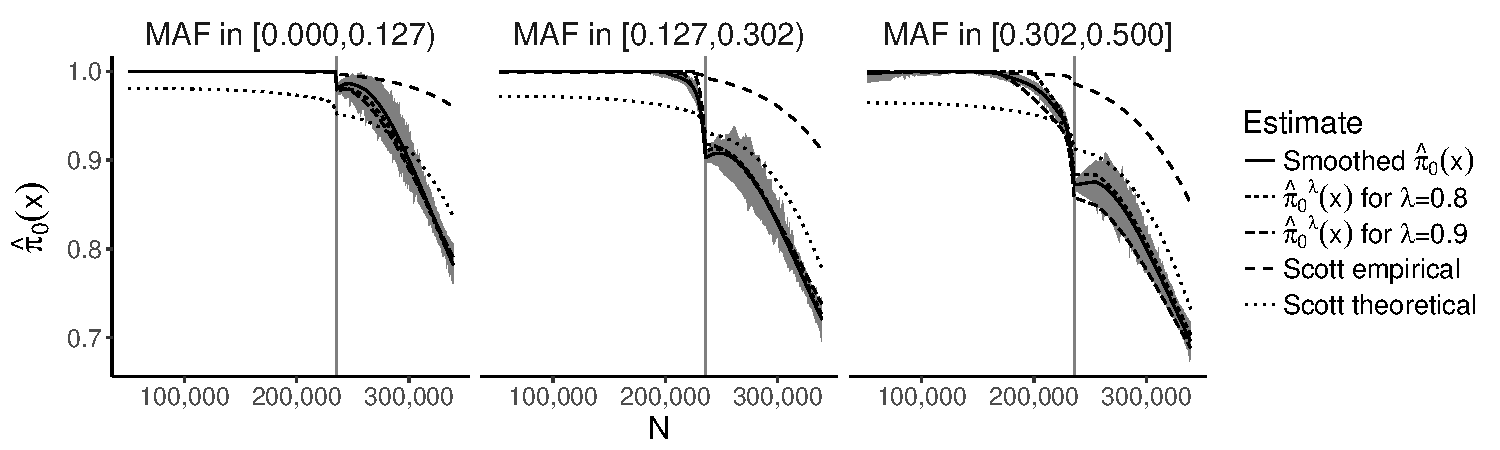
\includegraphics[scale=0.48]{Fig2-1.pdf} 
\end{center}

Grey = 90\% bootstrap CI \\
Vertical line = median sample size

\end{frame}

%%%%%%%%%%%%%%%%%%%%%%%%%
%%%%%%%%%%%%%%%%%%%%%%%%%
%%%%%%%%%%%%%%%%%%%%%%%%%

\begin{frame}
\frametitle{Approach: Use plug-in estimate of $\pi_0(\bx_i)$ for FDR$(\bx_i)$}

\begin{itemize}
\item Multiply estimate of FDR obtained via BH approach by our estimate of $\pi_0(\bx_i)$

\item Note that is the same as approach of Storey, but considers extension to covariates

\item Major assumption: Conditional on the null being true, the p-values do not depend on the covariates\\ \vspace{0.2cm}
i.e. the probability of a feature being from one of the two distributions depends on the covariates but the actual test statistic and p-value
does not depend on the covariates further under the null.
\end{itemize}

\end{frame}

%%%%%%%%%%%%%%%%%%%%%%%%%
%%%%%%%%%%%%%%%%%%%%%%%%%
%%%%%%%%%%%%%%%%%%%%%%%%%

\begin{frame}
\frametitle{Results for estimated FDR$(\bx_i)$ for BMI GWAS}

Number of  SNPs with an estimated FDR $\le5$\% for various approaches.

\begin{table}[ht]
\begin{tabular}{m{2.2cm}rrrrr}
  \hline
 & BL & Scott T & Scott E & Storey & BH \\ 
  \hline
Number with $\widehat{FDR} \le 5$\%  & 13,384 & 16,697 & 7,636 & 12,771 & 12,500 \\ 
   \hline
\end{tabular}
\end{table}

\vspace{0.5cm}
BL = our approach \\
Scott T = Scott et al approach with theoretical null \\
Scott E = Scott et al approach with empirical null \\

\vspace{0.5cm}
All the discoveries from the BH approach are also present in BL.\\
Overlap with Storey = 12,740.

\end{frame}

%%%%%%%%%%%%%%%%%%%%%%%%%
%%%%%%%%%%%%%%%%%%%%%%%%%
%%%%%%%%%%%%%%%%%%%%%%%%%

\begin{frame}
\frametitle{Simulations to check FDR control and power}

Extensive simulations are presented in our paper/Github page.\\ \vspace{0.2cm}
Power = TPR (true positive rate) = fraction of truly alternative discoveries out of the total number of truly alternative features. \\
\vspace{0.5cm}

\textbf{The good:}

\begin{itemize}
\item If there is no or low correlation between test statistics, generally shows good control of FDR
\item Always leads to an improvement in power over Benjamini-Hochberg, which increases with lower $\pi_0(\bx_i)$ (max 6\%-11\% in absolute terms)
\item Improved interpretability compared to Storey's approach
\item FDR control is much better compared to Scott FDR regression approach when test statistics are not from a normal distribution
\end{itemize}

\end{frame}

%%%%%%%%%%%%%%%%%%%%%%%%%
%%%%%%%%%%%%%%%%%%%%%%%%%
%%%%%%%%%%%%%%%%%%%%%%%%%

\begin{frame}
\frametitle{Simulations to check FDR control and power}

Extensive simulations are presented in our paper/Github page.\\ \vspace{0.2cm}
Power = TPR (true positive rate) = fraction of truly alternative discoveries out of the total number of truly alternative features. \\
\vspace{0.5cm}

\textbf{The caveats:}

\begin{itemize}
\item If test statistics are highly correlated, does not appropriately control the FDR
\item If $\pi_0(\bx_i)$ is high, not much gain in power over Benjamini-Hochberg
\item Gain in power over Storey's approach is usually minimal (0-2\%)
\item Power is better for Scott FDR regression approach when test statistics are from a normal distribution
\end{itemize}

\end{frame}

%%%%%%%%%%%%%%%%%%%%%%%%%
%%%%%%%%%%%%%%%%%%%%%%%%%
%%%%%%%%%%%%%%%%%%%%%%%%%

\begin{frame}
\frametitle{Conclusions}

We developed a direct approach to estimating FDR conditional on covariates. \vspace{0.5cm}

Why should you use it?
\begin{itemize}
\item Improved power compared to BH
\item Improved interpretability compared to Storey
\item Improved robustness compared to Scott
\end{itemize} \vspace{0.5cm}

We hope to extend/apply this approach to a number of other scenarios.

\end{frame}

%%%%%%%%%%%%%%%%%%%%%%%%%
%%%%%%%%%%%%%%%%%%%%%%%%%
%%%%%%%%%%%%%%%%%%%%%%%%%

\begin{frame}
\frametitle{Questions?}

Email: smb310@georgetown.edu \\ \vspace{0.2cm}

Twitter: \href{https://twitter.com/siminaboca}{@siminaboca} \\ \vspace{0.2cm}

Preprint: \url{http://www.biorxiv.org/content/early/2017/07/25/035675} \\ \vspace{0.2cm}

Code for all analyses/simulations in paper: \url{https://github.com/SiminaB/Fdr-regression} \\ \vspace{0.2cm}

Package which includes FDR regression approach: \url{https://bioconductor.org/packages/release/bioc/html/swfdr.html}\\
(uses linear, not logistic regression)

\end{frame}

\end{document}


%%%%%%%%%%%%%%%%%%%%%%%%%
%%%%%%%%%%%%%%%%%%%%%%%%%
%%%%%%%%%%%%%%%%%%%%%%%%%


\section{Multivariate meta-analysis}

\begin{frame}
\frametitle{\hfill}

\Huge
\begin{center}Multivariate meta-analysis\end{center}

\end{frame}

\begin{frame}
\frametitle{Multivariate meta-analysis}

In epidemiology, we often want to consider multiple risk factors
together, or multiple levels of a single exposure.

\vspace{0.5cm}

Can meta-analyze each parameter/coefficient separately,
but that may not be efficient!

\pause

\vspace{0.5cm}

The correlations between the coefficient estimates will allow
for borrowing of strength.

\end{frame}

%%%%%%%%%%%%%%%%%%%%%%%%%
%%%%%%%%%%%%%%%%%%%%%%%%%
%%%%%%%%%%%%%%%%%%%%%%%%%

\begin{frame}
\frametitle{InterLymph Consortium}

Interested in the following 4 associations with lymphoma:
\begin{enumerate}
\setlength{\itemindent}{0.2in}
\item Lifetime cigarette exposure as smoking pack-years.
\end{enumerate}
\hspace{0.1in}Number of servings per week of: 
\begin{enumerate} 
  \setcounter{enumi}{1}
\setlength{\itemindent}{0.5in}
\item wine
\item liquor
\item beer
\end{enumerate}

\vspace{0.3cm}

For $I=15$ studies, fit: \color{red}
\begin{eqnarray*}
logit[P(\mbox{lymphoma})] = \mu_0 + \mu_1 X_1 +\mu_2 X_2 + \mu_3 X_3 + \mu_4 X_4.
\end{eqnarray*}

\end{frame}


%%%%%%%%%%%%%%%%%%%%%%%%%
%%%%%%%%%%%%%%%%%%%%%%%%%
%%%%%%%%%%%%%%%%%%%%%%%%%

\begin{frame}
\frametitle{Multivariate meta-analysis}

For each study $1 \le i \le I$ there are $p$ coefficients which
need to be estimated:

\begin{itemize} 
\item \large$\bmu_i$ \normalsize is a vector which has the $p$ coefficients.
\[
\bmu_i =
\begin{bmatrix}
\mu_{1i} \\
\vdots \\
\mu_{pi}
\end{bmatrix}
\]
\item \large$\hat{\bmu}_i$ \normalsize is a vector of 
estimates for the $p$ coefficients in $\bmu_i$.
\[
\bY_i =
\begin{bmatrix}
Y_{1i} \\
\vdots \\
Y_{pi}
\end{bmatrix}
\]
\end{itemize}

\end{frame}

%%%%%%%%%%%%%%%%%%%%%%%%%
%%%%%%%%%%%%%%%%%%%%%%%%%
%%%%%%%%%%%%%%%%%%%%%%%%%

\begin{frame}
\frametitle{Multivariate meta-analysis}

A common assumption is:
\begin{eqnarray*}
\bY_i | \bmu_i \sim MVN(\bmu_i, \bS_i),
\end{eqnarray*}
where $\bS_i$ is the \color{red}within-study variance-covariance matrix.

\begin{itemize}
\item FE meta-analysis:
\begin{eqnarray*}
\bmu_i \equiv \bmu.
\end{eqnarray*}
\item RE meta-analysis:
\begin{eqnarray*}
\bmu_i \sim MVN(\bmu, \bSigma),
\end{eqnarray*}
where $\bSigma$ is the \color{red}between-study variance-covariance matrix.
\color{black}

\end{itemize}

\end{frame}

%%%%%%%%%%%%%%%%%%%%%%%%%
%%%%%%%%%%%%%%%%%%%%%%%%%
%%%%%%%%%%%%%%%%%%%%%%%%%

\begin{frame}
\frametitle{Multivariate meta-analysis}

The MVMA estimate of
$\bmu$ is:
\begin{eqnarray*}
\hat{\bmu}^M
&=& \left[\sum_{i=1}^I (\hat{\bS}_i+\hat{\bSigma})^{-1} \right]^{-1} \sum_{i=1}^I (\hat{\bS}_i+\hat{\bSigma})^{-1} \bY_i .
\end{eqnarray*}

The UVMA estimate of $\bmu$ is:
\begin{eqnarray*}
\hat{\bmu}^U &=& \left[\sum_{i=1}^I (\hat{\bU}_i+\hat{\bD})^{-1} \right]^{-1} \sum_{i=1}^I (\hat{\bU}_i+\hat{\bD})^{-1} \bY_i,
\end{eqnarray*}
where $\bU_i = diag(\bS_i)$ and $\bD = diag(\bSigma)$. 

 For the RE framework, we estimate the between-study variance-covariance matrix $\bSigma$ by restricted maximum likelihood (REML), implemented in the 
\texttt{mvmeta} R package.

\end{frame}


%%%%%%%%%%%%%%%%%%%%%%%%%
%%%%%%%%%%%%%%%%%%%%%%%%%
%%%%%%%%%%%%%%%%%%%%%%%%%

\section{Efficiency of multivariate vs. univariate meta-analysis}

\begin{frame}
\frametitle{\hfill}

\Huge
\begin{center}Efficiency of multivariate vs. univariate meta-analysis\end{center}

\end{frame}

%%%%%%%%%%%%%%%%%%%%%%%%%
%%%%%%%%%%%%%%%%%%%%%%%%%
%%%%%%%%%%%%%%%%%%%%%%%%%

\begin{frame}
\frametitle{Efficiency of multivariate vs. univariate meta-analysis}

Can consider their variances: \scriptsize \hspace{-0.1cm}
\[
Var\!\!\left(\hat{\bmu}^M\right)\! \approx \left[  \sum_{i=1}^I(\bS_i + \hat{\bSigma})^{-1} \right]^{-1} \]
\hspace{-0.9cm}\[
\!\!\!\!\!\!\!\!\!Var\!\!\left(\hat{\bmu}^U\right)\!\! \approx \!\! \left[\sum_{i=1}^I (\bU_i+ \hat{\bD})^{-1} \!\!\right]^{-1}\!\!\! 
\left[  \sum_{i=1}^I (\bU_i+\hat{\bD})^{-1}(\bS_i + \hat{\bSigma})(\bU_i+\hat{\bD})^{-1} \!\!\right]\!\!\!
\left[\sum_{i=1}^I (\bU_i+ \hat{\bD})^{-1}\!\!\right]^{-1} 
\]

\vspace{0.3cm}

\normalsize

We define the \color{red}relative efficiency \color{black} for $\hat{\mu}_k$, the $k^{th}$ parameter of $\hat{\bmu}$, to be 
\begin{eqnarray*}
	\label{RelEff}
\mbox{RelEff}_k := \frac{Var(\hat{\mu}^M_{k})}{Var(\hat{\mu}^U_{k})} 
\end{eqnarray*}

%We also discuss the estimates $\hat{\bmu}^{MT}$ and $\hat{\bmu}^{UT}$ that would be possible had the \textit{true} values of $\bSigma$ and $\bD$ been known and used

\end{frame}

%%%%%%%%%%%%%%%%%%%%%%%%%
%%%%%%%%%%%%%%%%%%%%%%%%%
%%%%%%%%%%%%%%%%%%%%%%%%%

\begin{frame}
\frametitle{Efficiency of multivariate vs. univariate meta-analysis}

We also discuss the estimates $\hat{\bmu}^{MT}$ and $\hat{\bmu}^{UT}$ that would be possible had the \textit{true} values of $\bSigma$ and $\bD$ been known and used:
\scriptsize \hspace{-0.1cm}
\[
Var\!\!\left(\hat{\bmu}^{MT}\right)\! = \left[  \sum_{i=1}^I(\bS_i + \bSigma)^{-1} \right]^{-1} \]
\hspace{-0.9cm}\[
\!\!\!\!\!\!\!\!\!Var\!\!\left(\hat{\bmu}^{UT}\right)\!\! = \!\! \left[\sum_{i=1}^I (\bU_i+ \bD)^{-1} \!\!\right]^{-1}\!\!\! 
\left[  \sum_{i=1}^I (\bU_i+ \bD)^{-1}(\bS_i + \bSigma)(\bU_i+ \bD)^{-1} \!\!\right]\!\!\!
\left[\sum_{i=1}^I (\bU_i+ \bD)^{-1}\!\!\right]^{-1} 
\]

\vspace{0.3cm}

\normalsize

We define the \color{red}relative efficiency \color{black} for $\hat{\mu}_k$ assuming the \color{red} true values of $\bSigma$ and $\bD$\color{black}, 
to be 
\begin{eqnarray*}
	\label{RelEff}
\mbox{RelEff}_k^T := \frac{Var(\hat{\mu}^{MT}_{k})}{Var(\hat{\mu}^{UT}_{k})} 
\end{eqnarray*}



\end{frame}

%%%%%%%%%%%%%%%%%%%%%%%%%
%%%%%%%%%%%%%%%%%%%%%%%%%
%%%%%%%%%%%%%%%%%%%%%%%%%

\begin{frame}
\frametitle{Relative efficiency for fixed effects case}

$I=2$ studies, $p=2$ parameters, $\bS_i = S^2\begin{pmatrix} 1 & \rho_i \\ \rho_i & 1 \end{pmatrix}$.

\begin{center}
\includegraphics[scale=0.55]{Figure_1_panel_a_edit.pdf} 
\end{center}

\vspace{-0.6cm}

\end{frame}

%%%%%%%%%%%%%%%%%%%%%%%%%
%%%%%%%%%%%%%%%%%%%%%%%%%
%%%%%%%%%%%%%%%%%%%%%%%%%

\begin{frame}
\frametitle{Relative efficiency for fixed effects case}

\vspace{0.1cm}

$I=2$ studies, $p$ parameters, $\bS_i = S^2\begin{pmatrix} 1 & \rho_i & ... & \rho_i \\ ... & ... & .... & ... \\ \rho_i & \rho_i & ... & 1 \end{pmatrix}$.

\begin{center}
\includegraphics[scale=0.55]{Figure_1_panel_b_edit.pdf} 
\end{center}

\vspace{-0.5cm}

\end{frame}


%%%%%%%%%%%%%%%%%%%%%%%%%
%%%%%%%%%%%%%%%%%%%%%%%%%
%%%%%%%%%%%%%%%%%%%%%%%%%

\begin{frame}
\frametitle{Relative efficiency for fixed effects case}

\vspace{0.1cm}

$I=20$ studies, $p$ parameters, $\bS_i = S^2\begin{pmatrix} 1 & \rho_i & ... & \rho_i \\ ... & ... & .... & ... \\ \rho_i & \rho_i & ... & 1 \end{pmatrix}$,
with $\rho_i = \rho(i-1)/20.$

\begin{center}
\includegraphics[scale=0.55]{Figure_1_panel_c_edit.pdf} 
\end{center}

\vspace{-0.5cm}

\end{frame}

%%%%%%%%%%%%%%%%%%%%%%%%%
%%%%%%%%%%%%%%%%%%%%%%%%%
%%%%%%%%%%%%%%%%%%%%%%%%%

\begin{frame}
\frametitle{Relative efficiency for random effects case assuming known variances}

\vspace{0.1cm}

$I=20$ studies, $p$ parameters, $\bS_i = S^2\begin{pmatrix} 1 & \rho_i & ... & \rho_i \\ ... & ... & .... & ... \\ \rho_i & \rho_i & ... & 1 \end{pmatrix}$,
 $\bSigma = \sigma^2\begin{pmatrix} 1 & 0.5 & ... & 0.5 \\ ... & ... & .... & ... \\ 0.5 & 0.5 & ... & 1 \end{pmatrix}$,
with $\rho_i = \rho(i-1)/20.$

\begin{center}
\includegraphics[scale=0.45]{Figure_2_panel_a_edit.pdf} 
\end{center}

\vspace{-0.6cm}

\end{frame}

%%%%%%%%%%%%%%%%%%%%%%%%%
%%%%%%%%%%%%%%%%%%%%%%%%%
%%%%%%%%%%%%%%%%%%%%%%%%%

\begin{frame}
\frametitle{Loss of efficiency when estimating variances versus knowing them}

\vspace{0.1cm}

$I=20$ studies, $p$ parameters, $\bS_i \approx S^2\begin{pmatrix} 1 & \rho_i & ... & \rho_i \\ ... & ... & .... & ... \\ \rho_i & \rho_i & ... & 1 \end{pmatrix}$,
 $\bSigma = \bzero$,
with $\rho_i = \rho(i-1)/20.$

\begin{center}
\includegraphics[scale=0.45]{Figure_2_panel_b_edit.pdf} 
\end{center}

\vspace{-0.6cm}

\end{frame}

%%%%%%%%%%%%%%%%%%%%%%%%%
%%%%%%%%%%%%%%%%%%%%%%%%%
%%%%%%%%%%%%%%%%%%%%%%%%%

\begin{frame}
\frametitle{Relative efficiency for random effects case: Known and estimated variances}

\vspace{0.1cm}

$I=20$ studies, $p$ parameters, $\bS_i \approx S^2\begin{pmatrix} 1 & \rho_i & ... & \rho_i \\ ... & ... & .... & ... \\ \rho_i & \rho_i & ... & 1 \end{pmatrix}$,
 $\bSigma = \bzero$,
with $\rho_i = \rho(i-1)/20.$

\begin{center}
\includegraphics[scale=0.45]{Figure_2_panel_c_edit.pdf} 
\end{center}

\vspace{-0.6cm}

\end{frame}


%%%%%%%%%%%%%%%%%%%%%%%%%
%%%%%%%%%%%%%%%%%%%%%%%%%
%%%%%%%%%%%%%%%%%%%%%%%%%

\begin{frame}
\frametitle{InterLymph data analysis}

\vspace{0.1cm}

Variables are highly correlated within studies and these correlations vary among studies, allowing opportunity to borrow information across parameters.



\begin{center}
\includegraphics[scale=0.45]{Figure_S1_edit.pdf} 
\end{center}

\end{frame}

%%%%%%%%%%%%%%%%%%%%%%%%%
%%%%%%%%%%%%%%%%%%%%%%%%%
%%%%%%%%%%%%%%%%%%%%%%%%%

\begin{frame}
\frametitle{InterLymph data analysis}

Estimates of log ORs (95\% confidence intervals) for lifestyle risk factors from the InterLymph consortium.

The wine, liquor, and beer variables are measured in servings per week/100, the smoking variable is measured in pack-years/100.

\begin{table}[ht] \small
\label{tab:InterLymph-all}
\begin{center}
\begin{tabular}{lcc}
  \hline
& \multicolumn{2}{c}{Fixed effects analysis} \\
Variable & MVMA & UVMA \\ 
  \hline
Wine & -0.33 (-0.67, 0.01) & -0.49 (-0.86, -0.12)  \\ 
  Liquor & -0.31 (-1.31, 0.69) & -0.18 (-1.26, 0.90) \\ 
  Beer & -0.82 (-1.38, -0.27) & -0.96 (-1.53, -0.40)  \\ 
  Smoking & 0.32 (0.17, 0.46) & 0.32 (0.18, 0.47) \\ 
   \hline
\end{tabular}
\end{center}
\end{table}

\end{frame}

%%%%%%%%%%%%%%%%%%%%%%%%%
%%%%%%%%%%%%%%%%%%%%%%%%%
%%%%%%%%%%%%%%%%%%%%%%%%%

\begin{frame}
\frametitle{InterLymph data analysis}

Estimates of log ORs (95\% confidence intervals) for lifestyle risk factors from the InterLymph consortium.

The wine, liquor, and beer variables are measured in servings per week/100, the smoking variable is measured in pack-years/100.

\begin{table}[ht] \small
\label{tab:InterLymph-all}
\begin{center}
\begin{tabular}{lcccc}
  \hline
& \multicolumn{2}{c}{Random effects analysis}\\
Variable & MVMA & UVMA\\ 
  \hline
Wine & -0.59 (-1.01, -0.18) & -0.49 (-0.86, -0.12) \\ 
  Liquor & 0.06 (-1.56, 1.68) & 0.26 (-1.39, 1.92) \\ 
  Beer & -0.75 (-1.48, -0.01) & -0.92 (-1.75, -0.09) \\ 
  Smoking & 0.26 (0.06, 0.47) & 0.26 (0.06, 0.46) \\ 
   \hline
\end{tabular}
\end{center}
\end{table}

\end{frame}

%%%%%%%%%%%%%%%%%%%%%%%%%
%%%%%%%%%%%%%%%%%%%%%%%%%
%%%%%%%%%%%%%%%%%%%%%%%%%

\begin{frame}
\frametitle{Simulations based on InterLymph data}

\begin{itemize}
\item Performed simulations where the within- and between- study correlation matrices are similar to those observed in InterLymph.
\item Considered $p=4$ risk factors similar to those in InterLymph.
\item Also considered $p=8$ risk factors, consisting of 2 blocks of 4 identically distributed risk factors based on InterLymph.
\begin{itemize}
\item Between-block correlations $\rho_{\bX}$ were considered to be either $0$ or $0.5$.
\item Blocks were taken to be independent in the between-study variance-covariance matrix.
\end{itemize}
\end{itemize}

\end{frame}

%%%%%%%%%%%%%%%%%%%%%%%%%
%%%%%%%%%%%%%%%%%%%%%%%%%
%%%%%%%%%%%%%%%%%%%%%%%%%

\begin{frame}
\frametitle{Simulations based on InterLymph data}

\begin{itemize}
\item Theory-based estimates of relative efficiency are similar to empirically observed estimates.
\item When $p=8$ and the correlation is non-negligible across variables ($\rho_{\bX}=0.5$), MVMA estimates may offer
substantial improvements.
\begin{itemize}
\item If the true model is FE and an FE model is fit, the empirical RelEff is between 0.57 and 0.81; if an RE model is fit, the empirical
RelEff is between 0.70 and 0.91.
\item If the true model is RE and an RE model is fit, the empirical RelEff is between 0.84 and 0.93, compared to the asymptotic RelEff$^T$, which is 
between 0.68 and 0.88.
\end{itemize}
\end{itemize}

\end{frame}


%%%%%%%%%%%%%%%%%%%%%%%%%
%%%%%%%%%%%%%%%%%%%%%%%%%
%%%%%%%%%%%%%%%%%%%%%%%%%

\section{Conclusions}

\begin{frame}
\frametitle{\hfill}

\Huge
\begin{center}Conclusions\end{center}

\end{frame}

\begin{frame}
\frametitle{Conclusions}

\begin{itemize}
\item In FE meta-analyses, the benefit from using MVMA can substantially increase as $p$ increases.
\item In RE meta-analyses, there is likely to be only a minimal efficiency gain when using MVMA instead of UVMA.
\item The efficiency gain is larger when the correlation structures vary across studies, but even in this case, the gain is small for RE.
\item Caveats of our study include not considering meta-analyses with missing estimates or correlations and only using REML estimation.
\item The maximal decrease in a parameter's variance in an RE meta-analysis is expected to be around 10\%, leading to a decrease in the confidence interval
of around 5\%; this needs to be weighted against the costs of the more complicated analysis in practice.
\end{itemize}

\end{frame}

\end{document}



